\section{Uczenie \texttt{dane\_sin1a}}

W następujących rysunkach są widoczne wykresy jak i błędy danych uczących na pliku \texttt{dane\_sin1a}. Zostały ustawione następujące wartości \texttt{spread}:
\begin{itemize}
\item 0.01
\item 0.06
\item 0.08
\item 1
\end{itemize}

Według wykresów błędu wynika że optymalna wartość \texttt{spread} jest 0.06.

\begin{figure}[!h]
\centering
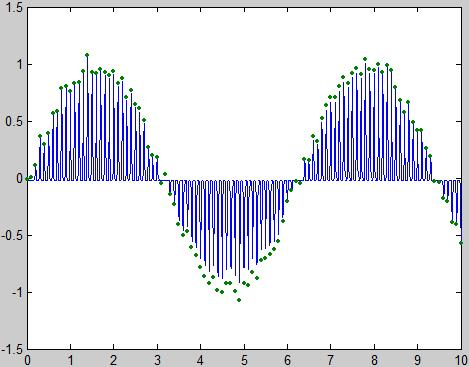
\includegraphics[scale=0.8]{src/0_01_wykres.png}\caption{\label{fig:0.01_wykres}Próbki (spread=0.01)}
\end{figure}

\begin{figure}[!h]
\centering
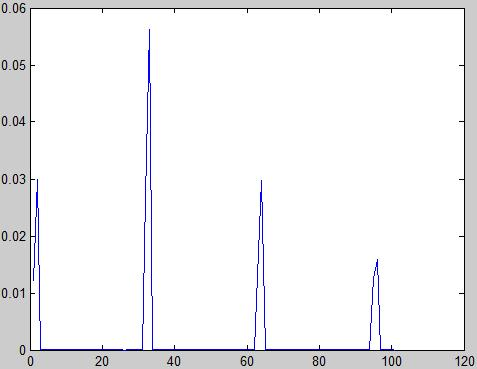
\includegraphics[scale=0.8]{src/0_01_blad.png}\caption{\label{fig:0.01_blad}Błąd (spread=0.01)}
\end{figure}

\begin{figure}[!h]
\centering
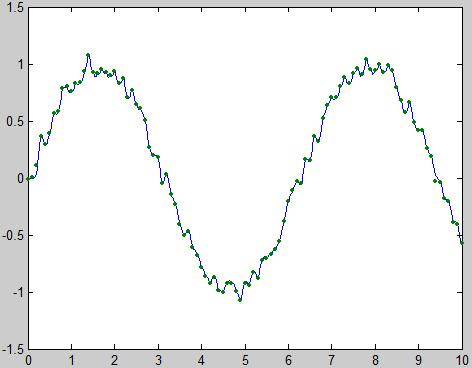
\includegraphics[scale=0.8]{src/0_06_wykres.png}\caption{\label{fig:0.06_wykres}Próbki (spread=0.06)}
\end{figure}

\begin{figure}[!h]
\centering
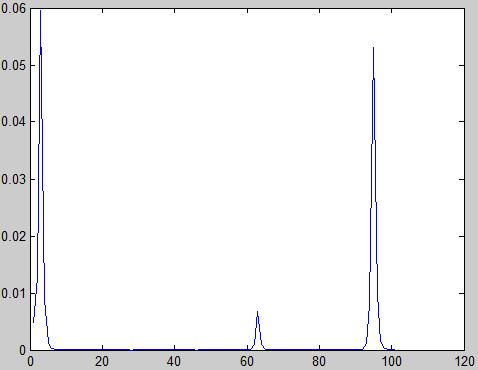
\includegraphics[scale=0.8]{src/0_06_blad.png}\caption{\label{fig:0.06_blad}Błąd (spread=0.06)}
\end{figure}

\begin{figure}[!h]
\centering
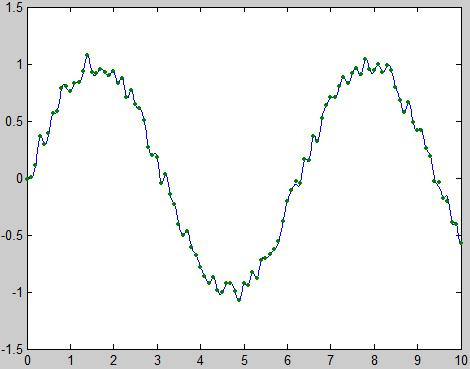
\includegraphics[scale=0.8]{src/0_08_wykres.png}\caption{\label{fig:0.08_wykres}Próbki (spread=0.08)}
\end{figure}

\begin{figure}[!h]
\centering
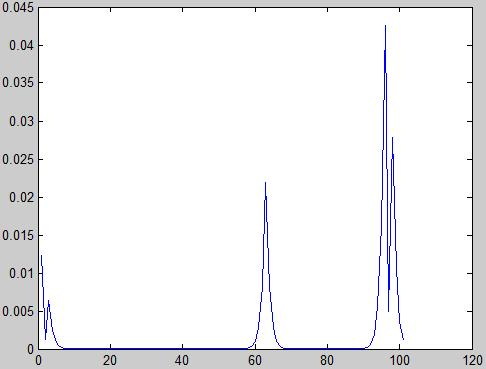
\includegraphics[scale=0.8]{src/0_08_blad.png}\caption{\label{fig:0.08_blad}Błąd (spread=0.08)}
\end{figure}

\begin{figure}[!h]
\centering
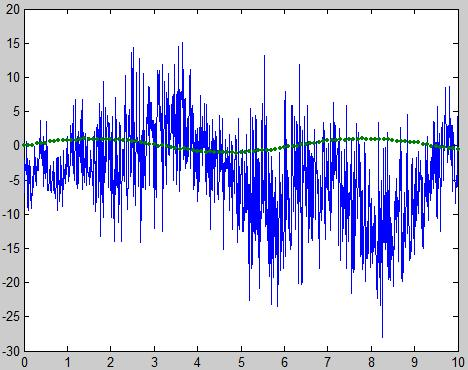
\includegraphics[scale=0.8]{src/1_wykres.png}\caption{\label{fig:0.08_wykres}Próbki (spread=1)}
\end{figure}

\begin{figure}[!h]
\centering
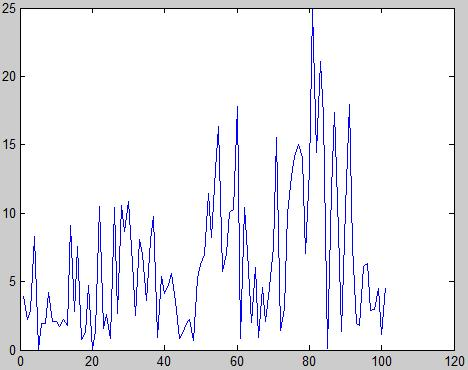
\includegraphics[scale=0.8]{src/1_blad.png}\caption{\label{fig:0.08_blad}Błąd (spread=1)}
\end{figure}

